\documentclass[11 pt, a4paper, twocolumn]{article}

% Fonts and math (Elsevier-like Times style)
\usepackage{newtxtext,newtxmath}
\usepackage{graphicx} % Required for inserting images
\usepackage{array} % For extra column formatting
\usepackage{amsmath} % for equation environment
\usepackage{float}
\usepackage{listings}
\usepackage{xcolor}
\usepackage{parskip} % For gaps between para
\usepackage{setspace}
\PassOptionsToPackage{hyphens}{url}\usepackage{hyperref}
\usepackage{makecell}
\usepackage[labelfont=bf]{caption}

% --- Abstract styling (elsarticle look)
\usepackage{abstract}
\renewcommand{\abstractnamefont}{\normalfont\bfseries}
\renewcommand{\abstracttextfont}{\normalfont}
\renewenvironment{abstract}{%
  \par\noindent\rule{\linewidth}{0.4pt}\par
  \begin{center}\bfseries Abstract\end{center}%
}{%
  \par\rule{\linewidth}{0.4pt}\par
}

% --- Section styling (similar to elsarticle)
\usepackage{titlesec}
\titleformat{\section}{\normalfont\large\bfseries}{\thesection.}{0.5em}{}
\titleformat{\subsection}{\normalfont\normalsize\bfseries}{\thesubsection.}{0.5em}{}

\title{\bfseries Orbits in the Solar System}
\author{Lian Fernandes}
\date{\today}

% --- Title info ---
\title{%

\includegraphics[width=0.9\linewidth]{UCD_Logo.png}\\ % Logo
{\large PHYC30170 Physics Astronomy and Space Lab I}\\ % Course info
{\bfseries Comparing Computational Methods for the Orbits in the Solar System} % Report title
}
\author{Lian Fernandes \\ \small Student No.: 22206311}
\date{09 September 2025}

% Python code export
\lstset{
    language=Python,
    basicstyle=\ttfamily\footnotesize,
    keywordstyle=\color{blue},
    commentstyle=\color{gray},
    stringstyle=\color{red},
    showstringspaces=false,
    frame=single,
    breaklines=true,
    numbers=left,
    numberstyle=\tiny\color{gray}
}

\begin{document}
\onecolumn
\maketitle


\begin{abstract}
Solving classcial n-body problems to determine the possible position and velocity of an object can be inefficient 
without the help of computational methods. Simulations of orbital systems in a single and binary star system were explored
using three numerical methods: Euler-Cromer, 2nd Order Runge-Kutta (RK2) and Leapfrog. Using Newton's and Kepler's Laws, circular
and elliptical orbits were reproduced in varying initial conditions and time steps. The Euler-Cromer was simple but less stable 
at larger time steps, while RK2 improved short term accuracy but lost stability over time. The Leapfrog method proved most effective
maintaining energy and angular momentum conservation over long simulations. Its symplectic nature makes it more reliable for
long-term orbit modelling. Future research could explore the effects of higher order integrators on complex n-body systems, thereby
improving accuracy and precision of celestial bodies.
\end{abstract}

\twocolumn

\section{Introduction}
Classical mechanics has been an intriguing field of study in physics, particularly due to its role in 
explaing the motion of the planets in the solar system. Some of the most fundamental concepts in 
classical mechanics are Newton's Law of Gravitation, the centripetal forces of orbits and Kepler's Laws 
(especially Kepler's Third Law). The complexity of the orbits in the solar system makes solving 
differential equations numerically challenging and tedious. However, applying numerical methods,
these equations can be solved with accuracy and efficiency, allowing for repeated computational analysis
and easier change in inital conditions as necessary.

With the advancement of science and technology, solving complex differential equations has become
manageable with the help of programming languages such as Python, C++, Java and more. In this paper, 
Python was used extensively, with libraries such as NumPy, SciPy, and Matplotlib supporting with 
analysis and visualisation. These tools make it easier to model the orbits of the solar system and
predict the behaviour and trajectories of the celestial objects in it. This experiment simulated the 
orbital motion of celestial bodies around the Sun using numerical methods (Euler-Cromer, 2nd order 
Runge-Kutta and Leapfrog method) and evaluated the accuracy of these methods under different conditions.

\subsection{Orbital Mechanics}
Orbital mechanics are modeled using Newton's gravitational law and laws of motion alongside Kepler's 
law of planetary motion. [1] Newton's gravitational law states that every object in the universe is
attracted to another object with force proportional to the product of their masses. [2] The equation 
that expresses this is

\[
F = G \frac{m_1m_2}{r^2}
\tag{Eq. 1a}
\]

where \textbf{F} is the gravitational force between the two objects, $m_1$ and $m_2$ are the masses 
of the two objects, \textit{r} is the distance between their centers, and \textit{G} is the 
gravitational constant ($6.674 \times 10^{-11}$ m$^3$kg$^-1$s$^-2$). 

In relation to our Solar System, the Sun is at the centre with celestial bodies (planets, comets, etc.)
revolving around it. Due to this, the equation becomes

\[
\mathbf{F} = -\frac{GmM}{|r|^3}\mathbf{r}
\tag{Eq. 1b}
\]

where \textit{M} is the mass of the Sun.

Applying Newton's second law of motion, $F=ma$, the acceleration of a celestial body, \textbf{a}(t),
can be expressed (assuming the Sun is stationary at the origin) as

\[
\mathbf{a}(t) = -\frac{GM}{|\mathbf{r}(t)|^3}\mathbf{r}(t)
\tag{Eq. 2}
\]

where $r = \sqrt{x^2 +y^2}$.
The negative sign indicates that the force is directed inwards to the Sun. Newton's third law, 
which states that every action has an equal and opposite reaction, is evident here. The gravitational 
force provides the centripetal force that keeps the body in orbit. [3] This relationship is expressed as
\[
\frac{GMm}{R^2} = \frac{mv^2}{R}
\tag{Eq. 3}
\]
where \textbf{R} is the radius of the orbit.

Although most celestial bodies have elliptical orbits, some bodies follow \textit{nearly} circular 
orbits. For circular orbits, the object's velocity, \textit{v}, is given by
\[
v = \sqrt{\frac{GM}{R}}
\tag{Eq. 4}
\]
to remain in a stable orbit.

Kepler's laws are just as fundamental to orbital mechanics as Newton's laws of motion. [4] They are 
stated as follows:
\begin{itemize}
    \item \textit{Kepler's First Law:} A planet's orbit around the Sun (due to the gravitational pull) 
    is an ellipse, with the Sun at one of the foci.
    \item \textit{Kepler's Second Law (Law of Equal Areas):} The line that joins the body and the Sun 
    sweeps out equal areas in equal time intervals.
    \item \textit{Kepler's Third Law:} The squares of the orbital periods of the planets are proportional
     to the cubes of their semi-major axes lengths.
\end{itemize}

In this experiment, Kepler's third law plays a big role in calculating the planet's trajectories. 
This is expressed as
\[
\left(\frac{P_1}{P_2}\right)^2 = \left(\frac{a_1}{a_2}\right)^3
\tag{Eq. 5}
\]
where $P$ is the period of the orbit in years and $a$ is the semi-major axis.

Along with the laws of motion, conversation of energy is fundamental in showing that an n-body system
maintains its orbits and its energy. Kinetic energy (KE) is the energy that the celestial body holds 
due to its motion, and is given by
\[
KE = \frac{1}{2}mv^2
\tag{Eq. 6}
\]
where $m$ is the mass of the body and $v$ is the total velocity in the $x$ and $y$ coordinates. 

The potential energy (PE) of the body is caused due to the planet's location in the system (being in the
same gravitational field of another body). [5] The equation is as Eq. 1b.

The sum of Kinetic and potential energy gives the total mechanical energy of the system.

For a binary system (two stars) with masses of $M_1$ and $M_2$, the acceleration of the body becomes
\[
\mathbf{a}(t) = -G\left(\frac{M_1}{(|r - r_1|)^3}(r - r_1) + \frac{M_2}{(|r - r_2|)^3}(r - r_2)\right)
\tag{Eq. 7}
\]
where $\mathbf{r_1}$ and $\mathbf{r_2}$ are the position of the two masses.

Energy is still conserved in such systems.

\subsection{Euler-Cromer Method}
The Euler-Cromer method is a modified version of the Euler method for solving ordinary dfferential 
equations (ODEs), particularly for various oscillatory and orbital systems. In orbital mechanics, 
this computes the vector position ($\mathbf{r}$) and the velocity, $\mathbf{v}$, of the body as

\begin{align}
\mathbf{v}(t+\Delta t) &= \mathbf{v}(t) + \Delta t\mathbf{a}(t) \tag{Eq. 8a}\\
\mathbf{r}(t+\Delta t) &= \mathbf{r}(t) + \Delta t\mathbf{v}(t+\Delta t) \tag{Eq. 8b}
\end{align}

where $\Delta t$ is the time step, $\mathbf{v}$ is the velocity vector, $\mathbf{r}$ is the position 
vector and $\mathbf{a}$ is the acceleration vector.

The updated velocity is used to compute the new position of the body, making the method more stable than
the standard Euler method. This preserves the total energy of the system over time, allowing the simulated 
bodies to stay in orbit for longer. [6], [7]

\subsection{Runge-Kutta Method}
The Runge-Kutta method is a family of numerical methods that approximates the solution to the ODE by
using the average of the slopes to extrapolate the solution. This includes the famously known 2nd order 
Runge-Kutta (RK2) and 4th order Runge-Kutta (RK4) methods. These methods predict the value first and 
then correct the solution based on additional slope information. [8] 

RK2 is a midpoint method that computes the acceleration of the body at the current step to estimate the 
velocity and position and evaluate the acceleration again at the midpoint. The midpoint slope is then used
to update the velocity and position.

For a system of the form $\dot{y} = f(t,y)$, RK2 is expressed as:
\vspace{-0.1em}
\begin{align}
k_1 &= f(t_n, y_n) \tag{Eq. 9a} \\
y_{mid} &= y_n + \frac{\Delta t}{2}k_1 \tag{Eq. 9b} \\
k_2 &= f(t_n + \frac{\Delta t}{2}, y_{mid}) \tag{Eq. 9c} \\
y_{n+1} &= y_n + \Delta t k_2 \tag{Eq. 9d}
\end{align}

where $k_1$ is the slope at the start of the interval, $y_{mid}$ is the midpoint value, $k_2$ is the 
slope at the midpoint and $\Delta t$ is the time step size.

Compared to the Euler-Cromer method, RK2 is greater in accuracy as it takes into consideration the 
information at the midpoint. However, like the Euler-Cromer method, it is not suitable for long-term
stability of orbit simulation. Over extended periods, the body would be out of its orbit (may spiral out)
as numerical errors accumulate. [8]

\subsection{Leapfrog Integration Method}
The Leapfrog integration method is quite similar to the velocity Verlet method where differential
equations is solved by calculating the position and velocity at staggered times. The equations are 
as follows:

\begin{align}
v(t +\frac{1}{2}\Delta t) &= v(t) + \frac{1}{2}a(t)\Delta t \tag{Eq. 10a} \\
r(t + \Delta t) &= r(t) + v(t +\frac{1}{2}\Delta t)\Delta t \tag{Eq. 10b} \\
v(t +\Delta t) &= v(t +\frac{1}{2}\Delta t) + \frac{1}{2}a(t + \Delta t)\Delta t \tag{Eq. 10c}
\end{align}

The positions and velocities are evaluated at half-integer time steps whereas the positions are 
calculated at full time steps. [9] This staggered computation improves numerical stability and
ensures better conservation of energy and angular momentum.

With it taking multiple steps at staggered intervals, this can be remain accurate for longer periods
of time, making it well-suited for orbital mechanics and n-body problems where long-term integration is needed.

\section{Methodology}
The equations for the different integration methods were defined, and initial conditions (initial 
velocity and position) were assigned. The simulation was carried out using astronomical units (AU) for
position and years (yr) for time. The unit of velocity is then expressed as AU/yr. The gravitational
constant simplifies to $G = 4 \pi^2$ and the solar mass is $M = 1$, allowing for straightforward
calculations. For circular orbits, the distance between the Sun and the object was fixed at 1 AU.

The Sun was placed at the origin (0,0) of the coordinate system. The body was initialized at
position (1,0), with a varying velocity to generate circular and elliptical orbits.

Equation (2) was used to determine the motion of the object. At each step of the simulation, a 
numerical integration method was applied to update the position and velocity of the object in discrete 
time step, $\Delta t$. The three numerical methods used were Euler-Cromer, 2nd Order Runge-Kutta and 
Leapfrog.

The Euler-Cromer method updates the velocity of the body first using the acceleration. The updated
velocity is then used to compute the new position. This process is repeated iteratively for the duration
of the simulation. This simple method however leads to large errors over a period of time.

The 2nd Order Runge-Kutta method computes the acceleration of the body at the current position and 
then estimates the velocity and position at the midpoint. The midpoint at the acceleration is then 
recalculated and used to update the velocity and position. This reduces the error when compared to 
the Euler-Cromer method but does not conserve the energy at large timescales.

The Leapfrog method computes the position and velocity at full-integer steps and half-integer steps
respectively. The velocity at the half-step is used to calulated the new position which is then used to
calculate the new acceleration. This is then looped until the required period is reached. Leapfrog is
more stable and conserves energy and angular momentum at longer periods.

Python was used to simulate the orbits, with the NumPy for numerical calulations and Matplotlib for the
graphical visualisation of the orbits. Position and velocity values at each time step were stored in
lists and later used to analyze the orbit dynamics. To get a quantitative analysis of the orbit and energy
conservation, the energy-time graph was created for each method. This was repeated to the 3-body problem: 
two stars of 0.5 solar masses at 0.4 AU apart and celestial body orbiting in the binary system.

\section{Results}
\textit{The complete set of graphs is provided in Appendix NO. These confirm the same trends as 
represented in this section.}

\subsection{Comparison of Numerical Methods}
\subsubsection{Circular Orbits}
The three numerical methods used to model the orbits of the solar system were Euler-Cromer, 
2nd Order Runge-Kutta (RK2) and Leapfrog. The initial conditions for the orbital simulations 
were set to $x = 1$ AU and $v_y=2\pi$ AU/yr. These were tested across all methods.

Figure 1 shows the circular orbit created using the Euler-Cromer method.
\begin{figure}[H]
  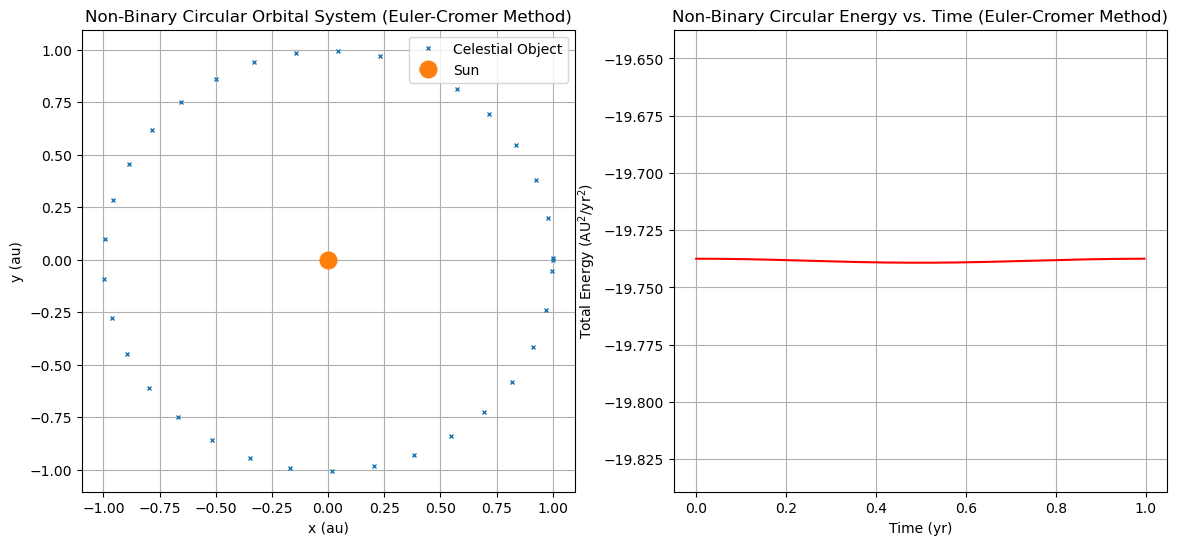
\includegraphics[width=1\linewidth]{Euler cromer/eulercromercircular.png}
  \centering
  \caption{\textit{Circular orbit of the object with $x = 1$ AU and $v_y = 2\pi$ AU/yr using 
  the Euler-Cromer method, with its corresponding energy-time graph.}} 
\end{figure}
\vspace{-3em}
The orbit plot clearly demonstrates a circular trajectory with a radius of 1 AU. However, the 
corresponding energy-time graph shows a slight dip, indicating that this method does not strongly 
conserve energy over a long period of time. 

Figure 2 shows the orbit generated using the RK2 method.
\begin{figure}[H] 
  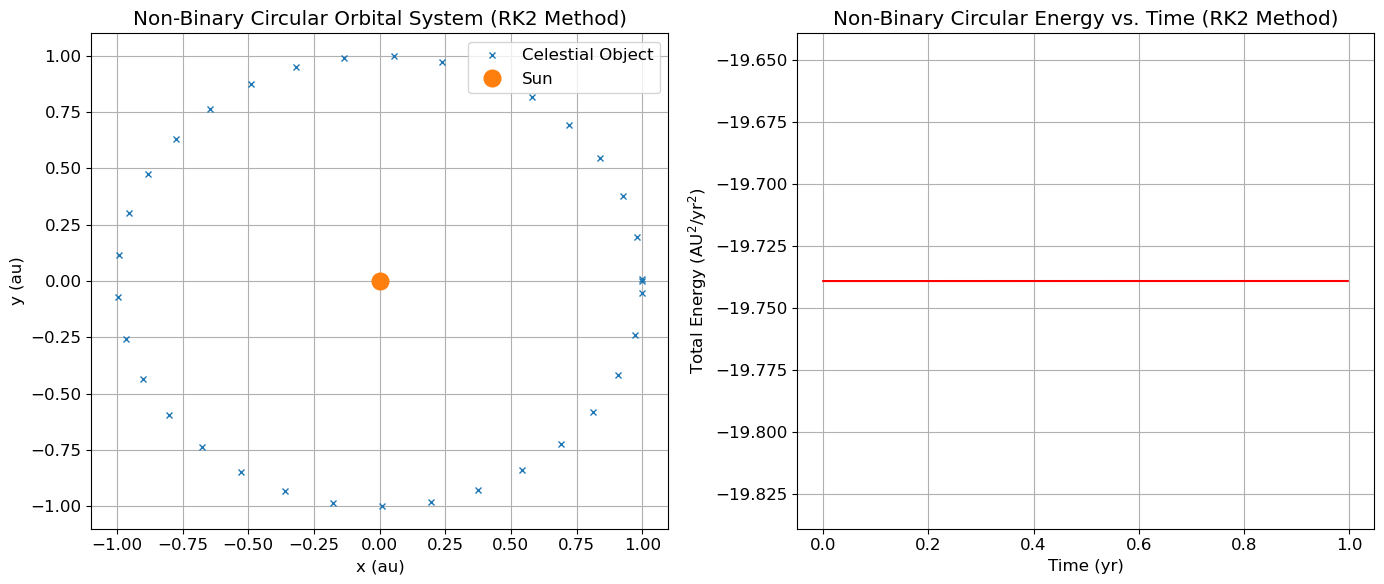
\includegraphics[width=1\linewidth]{RK2/rk2circular.png}
  \centering
  \caption{\textit{Circular orbit of the object with $x = 1$ AU and $v_y = 2\pi$ AU/yr using the RK2 
  method, with its corresponding energy-time graph.}}
\end{figure}
\vspace{-3em}
Here, the orbit remains circular with the radius of 1 AU, and the energy-time graph forms a nearly 
straight line. This suggests that, in constrast to Euler-Cromer, RK2 conserves energy more effectively
under these conditions.

Figure 3 illustrates the orbit created using the Leapfrog method.
\begin{figure}[H]
  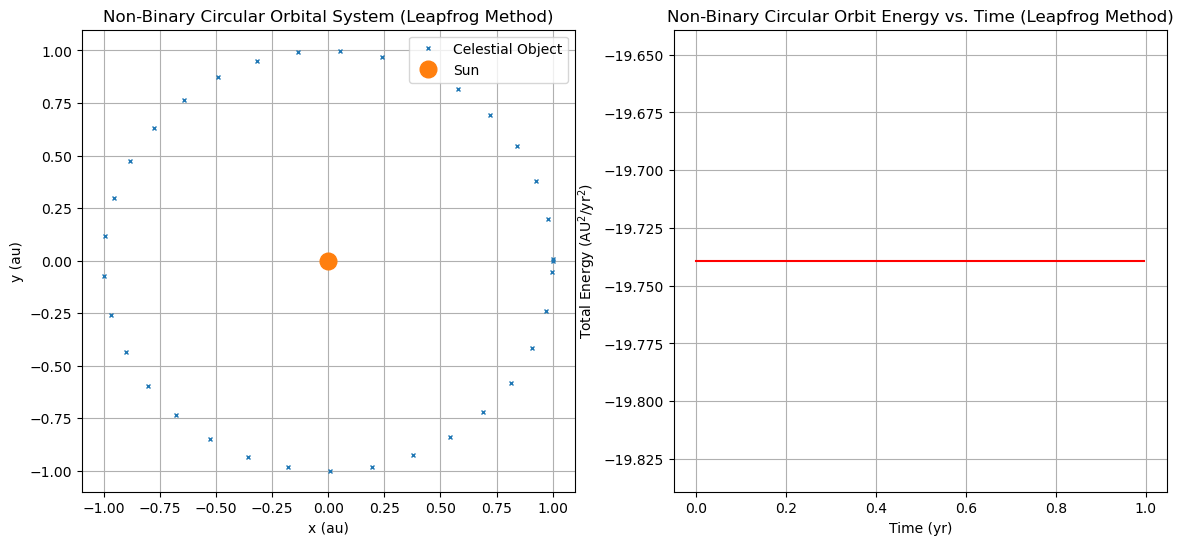
\includegraphics[width=1\linewidth]{Leapfrog/leapfrogcircular.png}
  \centering
  \caption{\textit{Circular orbit of the object with $x = 1$ AU and $v_y = 2\pi$ AU/yr using the 
  Leapfrog method with its corresponding energy-time graph.}}
\end{figure}
\vspace{-1em}
The trajectory again forms circle with a radius of 1 AU. Similar to RK2, the Leapfrog method produces an
energy-time graph that is essentially a straight line, indicating strong conservation of energy.

\subsubsection{Elliptical Orbits}
The same numerical methods were also applied to elliptical orbits of the object orbiting in a non-binary
system. The inital conditions for these simulations were $x=1$ AU and $v_y = \pi$ AU/yr.

Figure 4 shows the elliptical orbit of the object produced using the Euler-Cromer method.
\begin{figure}[H]
  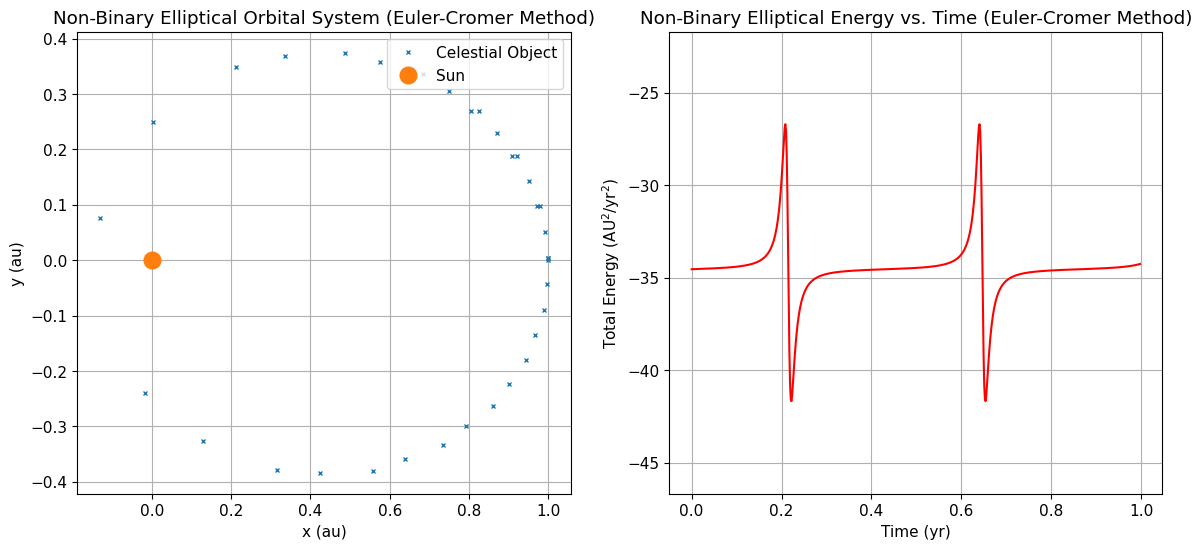
\includegraphics[width=1\linewidth]{Euler cromer/eulercromerelliptic.png}
  \centering
  \caption{\textit{Elliptical orbit of the object with $x = 1$ AU and $v_y = \pi$ AU/yr using the 
  Euler-Cromer method, with the corresponding energy-time graph.}} 
\end{figure}
\vspace{-1.5em}
The orbit plot shows an elliptical trajectory with noticeable deviations after a certain period. This
instability is reflected on the energy-time graph, showing energy fluctuations before stabilising again.
The oscillating energy created this tangential graph, showing energy is not conserved over time.

Figure 5 presents the simulation obtained using the RK2 method.
\begin{figure}[H]
  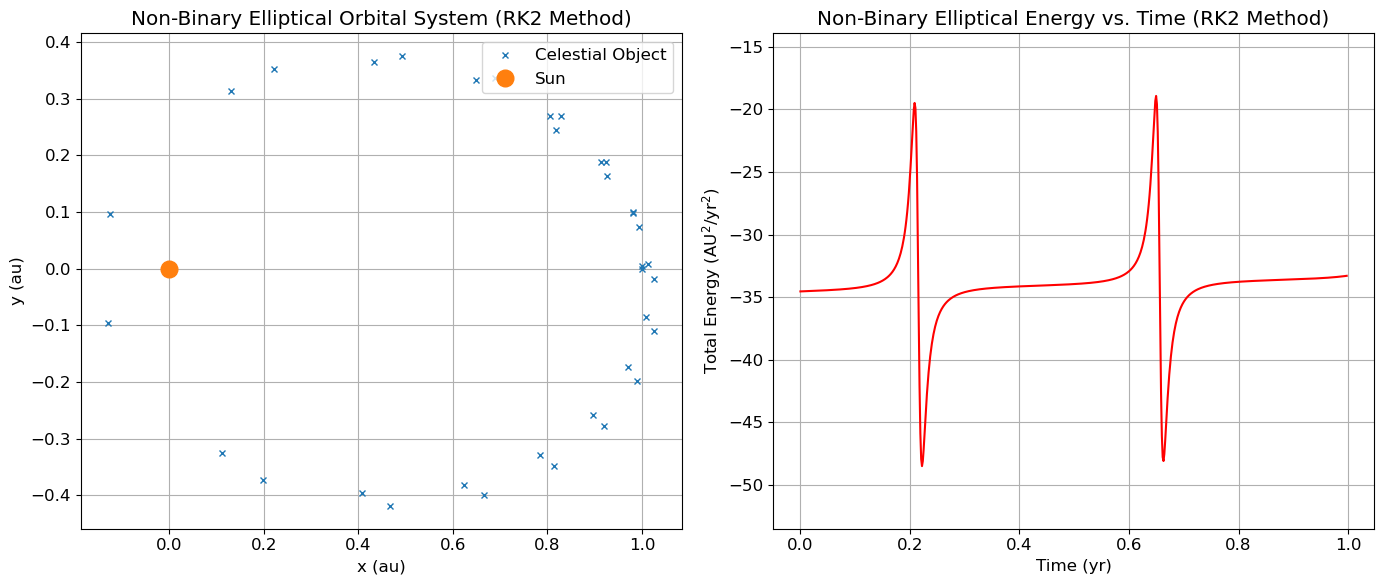
\includegraphics[width=1\linewidth]{RK2/rk2elliptic.png}
  \centering
  \caption{\textit{Elliptical orbit of the object with $x = 1$ AU and $v_y = \pi$ AU/yr using the RK2 
  method, with its corresponding energy-time graph.}} 
\end{figure}
\vspace{-1.5em}
The orbit maintains an overall elliptical shape orbit with a lot of deviations over time. The 
energy-time graph also shows these deviations with the maximum energy at approximately 
-20 AU$^2$/yr$^2$ and the minimum energy at approximately -47 AU$^2$/yr$^2$. The graph also follows the same pattern of the 
Euler-Cromer method, with a tangential graph showing the difting of the energy.

Figure 6 shows the elliptical orbit of the object created using the Leapfrog method.
\begin{figure}[H]
  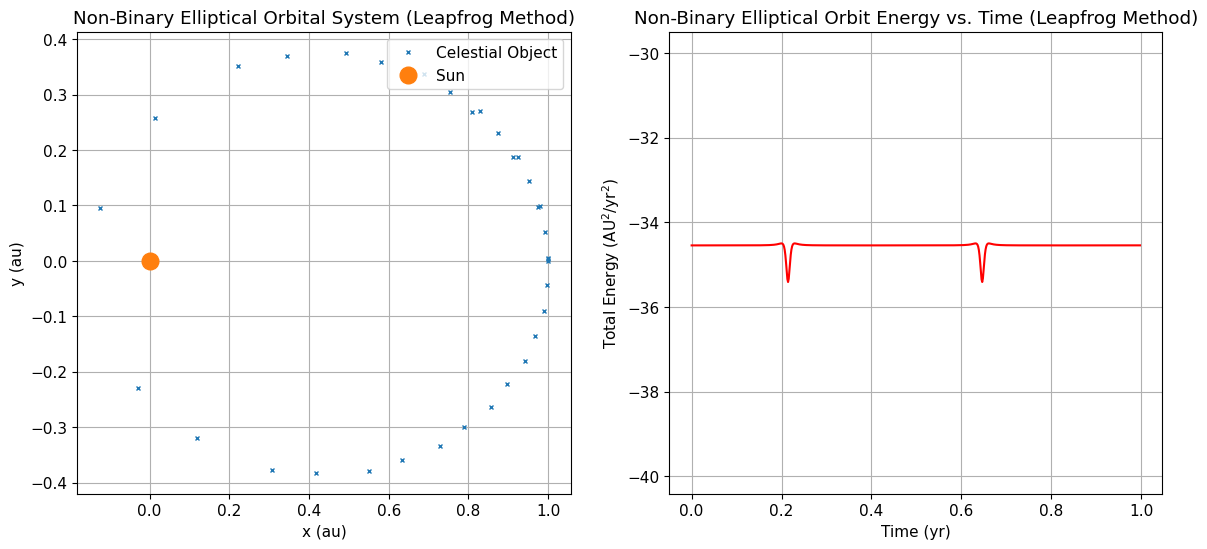
\includegraphics[width=1\linewidth]{Leapfrog/leapfrogelliptic.png}
  \centering
  \caption{\textit{Elliptical orbit of the object with $x = 1$ AU and $v_y = \pi$ AU/yr using the
   leapfrog method and the energy-time graph.}} 
\end{figure}
\vspace{-1.5em}
The Leapfrog method produces a stable elliptical orbit with minimal deviations over time. 
This is supported by the energy-time graph which was nearly constant with small oscillations at certain
times.

These results show that for an elliptical orbit, the Leapfrog method preserved energy more effectively than
the Euler-Cromer and RK2 method for longer integrations.

\subsection{Effect of Time Step}
In this section, for all methods, the time step, $dt$, was changed from 0.0015 (Figures 1 to 6) to 0.015, as an increase in the time step. Due less numbers being computed with this time step, 
the number of shapshots were increased from 20 to 2, allowing more values to be plotted on the graph and be calcuated. This means that every second value of the computed values were now being plotted and calcuated.

\subsubsection{Circular Orbits}
The same numerical methods were applied again. The variable that was changed was the number of 
snapshots as shown in the plots.

Figure 7 shows the circular orbit of the object created using the Euler-Cromer method 
with an increased time step.
\begin{figure}[H]
  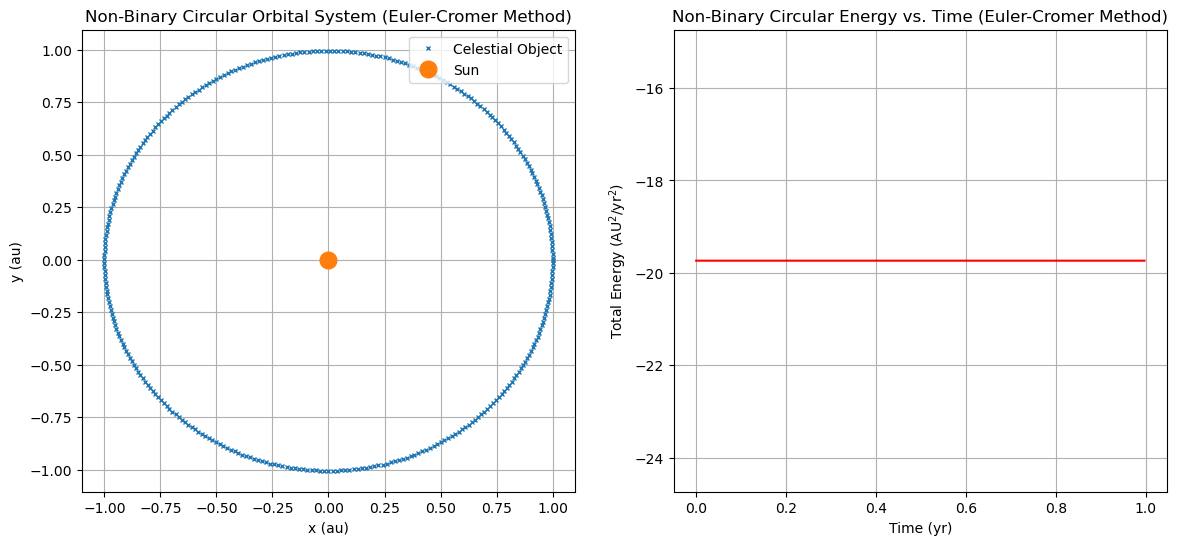
\includegraphics[width=1\linewidth]{Euler cromer/eulercromercircularincrease.png}
  \centering
  \caption{\textit{Circular orbit of the object with $x = 1$ AU and $v_y = 2\pi$ AU/yr using the 
  Euler-Cromer method, with an increased number of snaps and a larger time step, along with its
  energy-time graph.}} 
\end{figure}
The orbit plot shows that the Euler-Cromer method has maintained the circular shape of the trajectory
with a radius of 1 AU. Similar to the results in Section 3.3.1, a small dip in energy in the
energy-time graph, showing that energy is not fully conserved using this method.

Figure 8 shows the circular orbit of the oject produced using the RK2 method with an increased time 
step and number of snapshots.
\begin{figure}[H]
  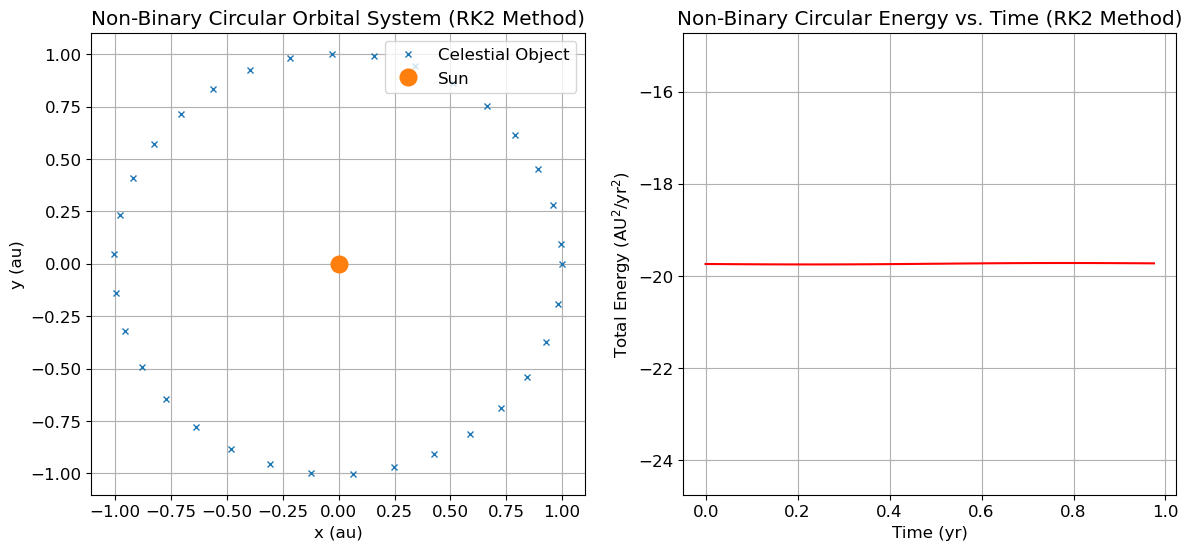
\includegraphics[width=1\linewidth]{RK2/rk2circularincrease.png}
  \centering
  \caption{\textit{Circular orbit of the object with $x = 1$ AU and $v_y = 2\pi$ AU/yr using the
  RK2 method with increased time steps and snapshots, along with its corresponding energy-time graph.}} 
\end{figure}
\vspace{-1em}
The RK2 method preserved the circular shape of the orbit under these conditions. The corresponding 
energy-time graph is not as conserved as the Euler-Cromer method.

Figure 9 shows the circular orbit of the object computed using the Leapfrog method, also with an increased
time step and number of snapshots.
\begin{figure}[H]
  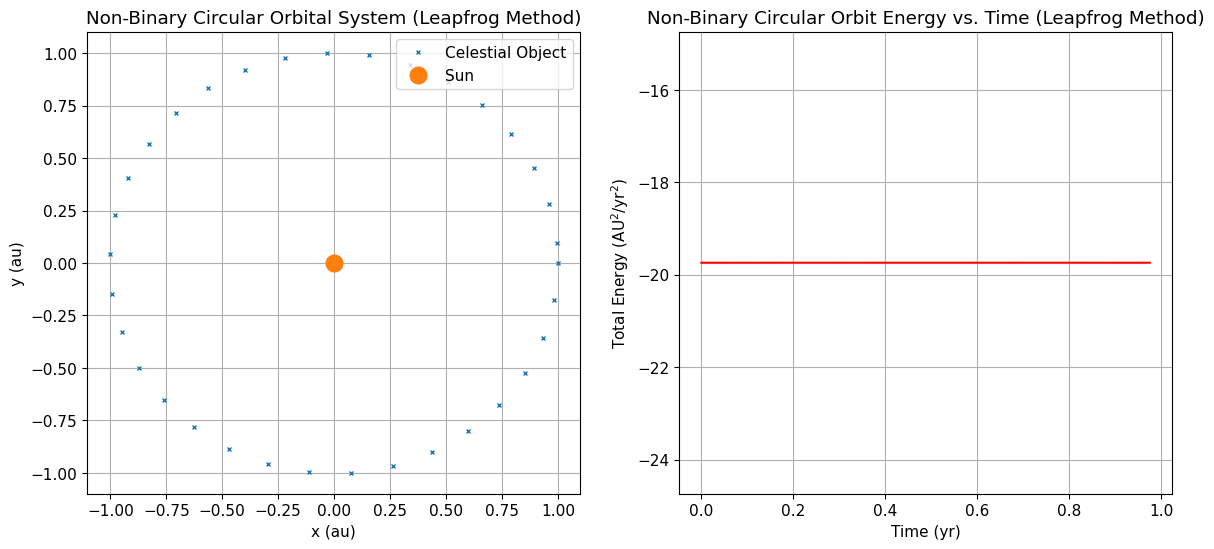
\includegraphics[width=1\linewidth]{Leapfrog/leapfrogcircularincrease.png}
  \centering
  \caption{\textit{Circular orbit of the object with $x = 1$ AU and $v_y = 2\pi$ AU/yr using the 
  Leapfrog method with increased time steps and snapshots, along with its corresponding energy-time graph.}} 
\end{figure}
\vspace{-1em}
The Leapfrog method maintained the circular stable orbit under the initial conditions. The energy-time
graph shows a straight line, preserving the energy.

\subsubsection{Elliptical Orbits}
Figure 10 shows the graph of an elliptical orbit using the Euler-Cromer method with an increased time
step and number of snapshots.
\begin{figure}[H]
  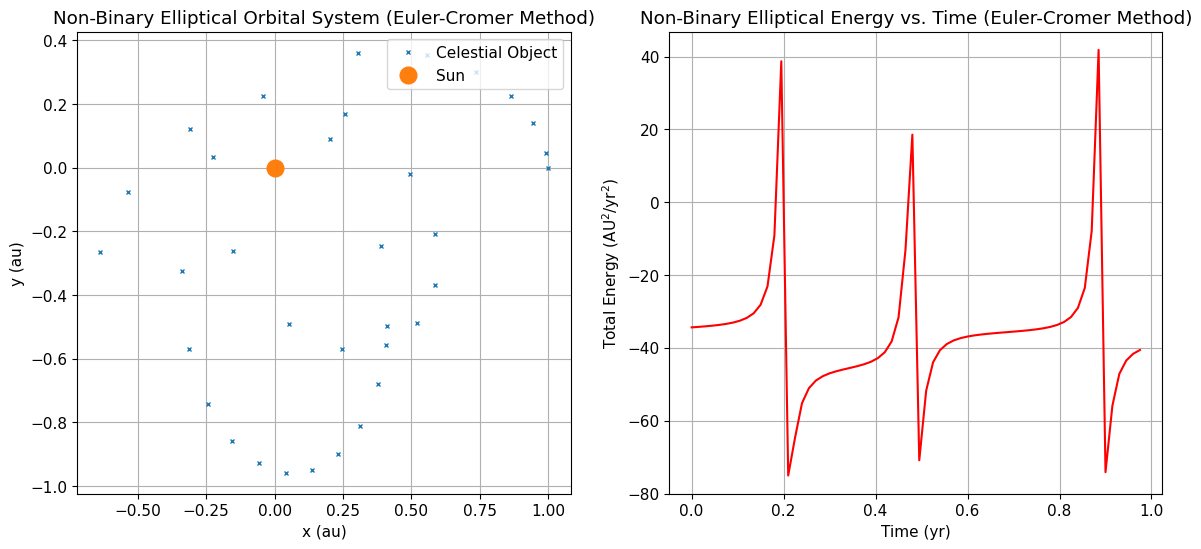
\includegraphics[width=1\linewidth]{Euler cromer/eulercromerellipticincrease.png}
  \centering
  \caption{\textit{Elliptical orbit of the object with $x = 1$ AU and $v_y = \pi$ AU/yr using the 
  Euler-Cromer method with increased snapshots and time stepm, along with its energy-time graph.}} 
\end{figure}
\vspace{-1em}
The plot appears chaotic and uneven under this method. The reduced resolution due to the large time step
gives inaccurate position updates, causing the trajectory to deviate significantly. The energy-time graph
shows large fluctuations, indicating the orbit is unstable and energy is not conserved.

Figure 11 shows the elliptical orbit of the object using the RK2 method with increased time steps and
snapshots.
\begin{figure}[H]
  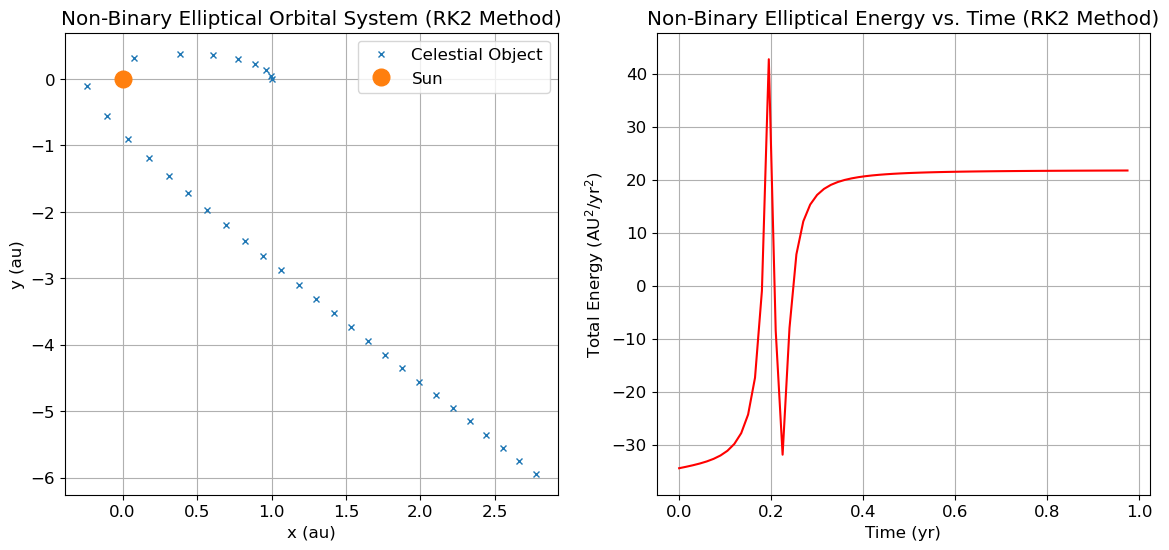
\includegraphics[width=1\linewidth]{RK2/rk2ellipticincrease.png}
  \centering
  \caption{\textit{Elliptical orbit of the object with $x = 1$ AU and $v_y = \pi$ AU/yr using the
  RK2 method with increased time steps and snapshots, along with its energy-time graph.}} 
\end{figure}
The orbit initially is elliptical in shape but quickly begins to spiral out, indicating instability.
This distortion is reflected in the energy-graph, showing rapid oscillations followed by a drift to
an incorrect energy value once the object leaves the orbit.

Figure 12 shows the elliptical orbit produced using the Leapfrog method with increased time steps
and snapshots.
\begin{figure}[H]
  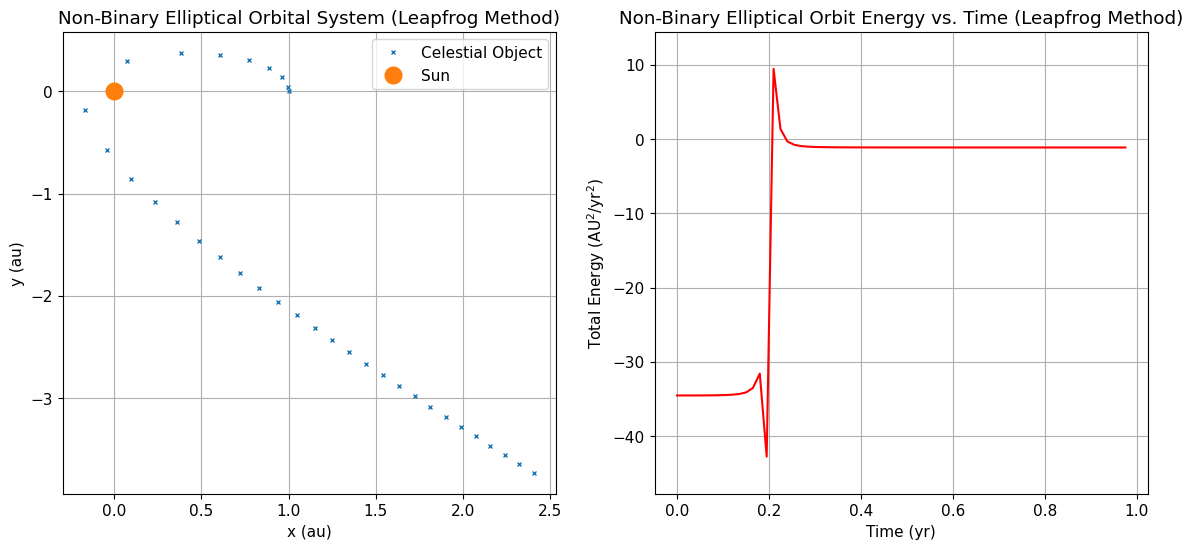
\includegraphics[width=1\linewidth]{Leapfrog/leapfrogellipticincrease.png}
  \centering
  \caption{\textit{Elliptical orbit of the object with $x = 1$ AU and $v_y = \pi$ AU/yr using the 
  Leapfrog method with increased time steps and snaps, along with its energy-time graph.}} 
\end{figure}
\vspace{-3em}
Similar to the RK2 results, the Leapfrog method initially produces a stable elliptical orbit but then
eventually spirals outward. The energy-time graph shows the same with constant energy before the object
drifts out of orbit.
\vspace{-2em}

\subsection{Numerical Integration on a Binary System}
Another star was added to the system to see the effects of the numerical methods on a binary system. The mass of the stars were 0.5 solar masses each, giving the system a total mass of 1 solar mass.
\vspace{-3em}
\subsubsection{Circular Orbits}
Figure 13 shows the binary system with a circular orbit of an object orbiting using the Euler-Cromer 
method.
\begin{figure}[H]
  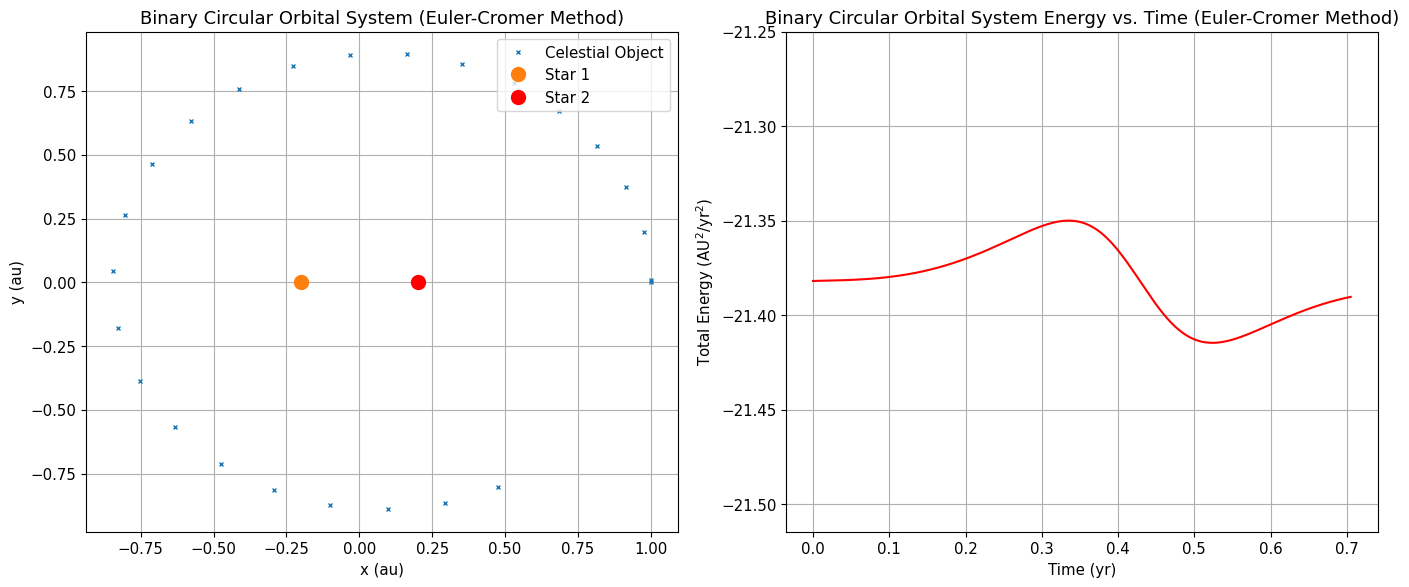
\includegraphics[width=1\linewidth]{binaryeulercircular.png}
  \centering
  \caption{\textit{Binary circular orbit of the object with $x = 1$ AU and $v_y = 2\pi$ AU/yr using 
  the Euler-Cromer method, with its corresponding energy-time graph.}} 
\end{figure}
\vspace{-1.5em}
The orbit plot shows a clear and stable circular orbit, indicating that the Euler-Cromer method performed
well in this system. The energy-time graph shows small fluctuations are around the theoretical energy 
value. However, these variations are minimal, suggesting most of the energy has been conserved in this 
system.

Figure 14 presents the binary system simulated using the RK2 method.
\begin{figure}[H]
  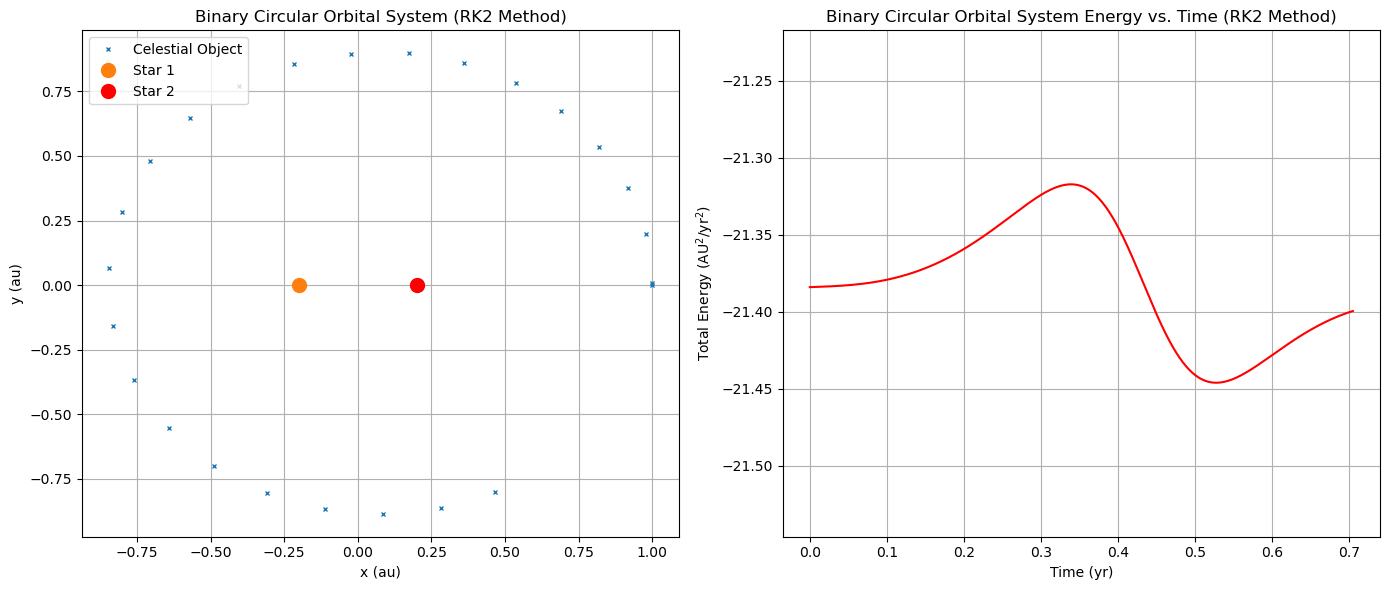
\includegraphics[width=1\linewidth]{binaryrk2circular.png}
  \centering
  \caption{\textit{Binary circular orbit of the object with $x = 1$ AU and $v_y = 2\pi$ AU/yr using the 
  RK2 method, with its corresponding energy-time graph.}} 
\end{figure}
\vspace{-1.5em}
Similar to the Euler-Cromer results, the graph keeps the circular shape, and the energy-time graph
shows slight fluctuations around the theoretical energy value.

Figure 15 shows the binary system modeled using the Leapfrog method.
\begin{figure}[H]
  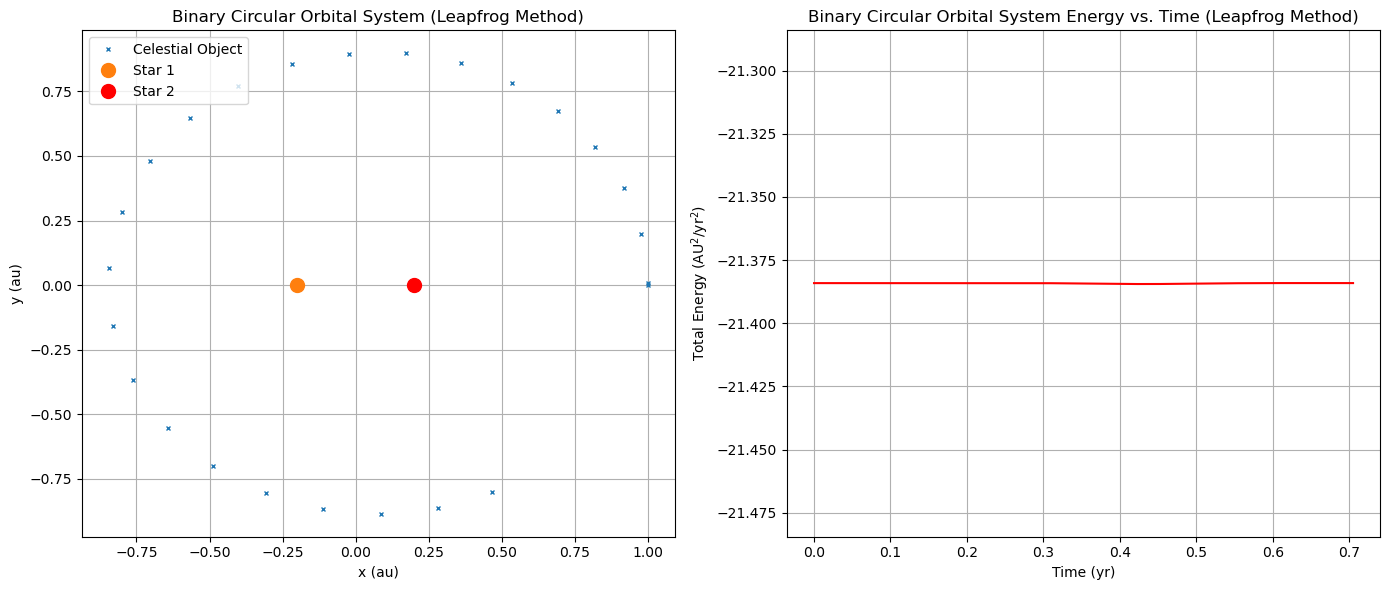
\includegraphics[width=1\linewidth]{binaryleapfrogcircular.png}
  \centering
  \caption{\textit{Binary circular orbit of the object with $x = 1$ AU and $v_y = 2\pi$ AU/yr using
  the Leapfrog method, with its corresponding energy-time graph.}} 
\end{figure}
The orbit again displays a stable circular shape consistent with the other methods. The energy-time 
graph shows a nearly straight line, indicating both and angular momentum are well conserved over the long 
periods of time.

\subsubsection{Elliptical Orbits}
Figure 16 shows the elliptical orbit of an object around a binary system computed using the Euler-Cromer
method.
\begin{figure}[H]
  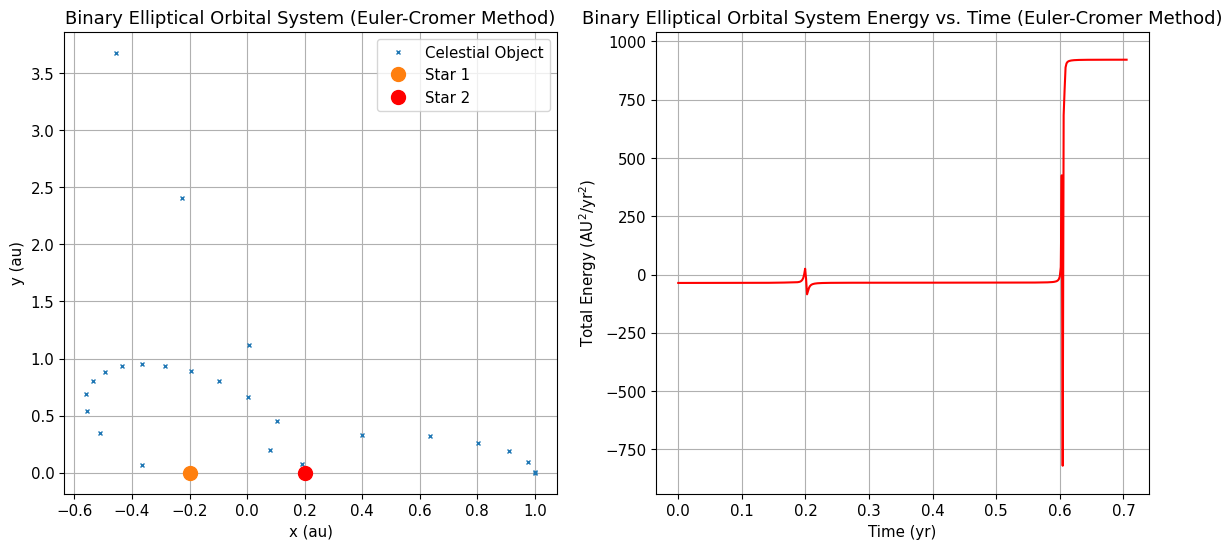
\includegraphics[width=1\linewidth]{binaryeulerelliptic.png}
  \centering
  \caption{\textit{Binary elliptical orbit of the object with $x = 1$ AU and $v_y = \pi$ AU/yr using
   the Euler-Cromer method with its corresponding energy-time graph.}} 
\end{figure}
The object initially orbits around both starss uniformally, maintaining the elliptical trajectory. 
However, after a certain period, the orbit becomes unstable and drifts away from the binary system. The
energy-time graph shows this instability, showing a significant displacement around 0.6 years.

Figure 17 shows the elliptical orbit of the object in the binary system using the RK2 method.
\begin{figure}[H]
  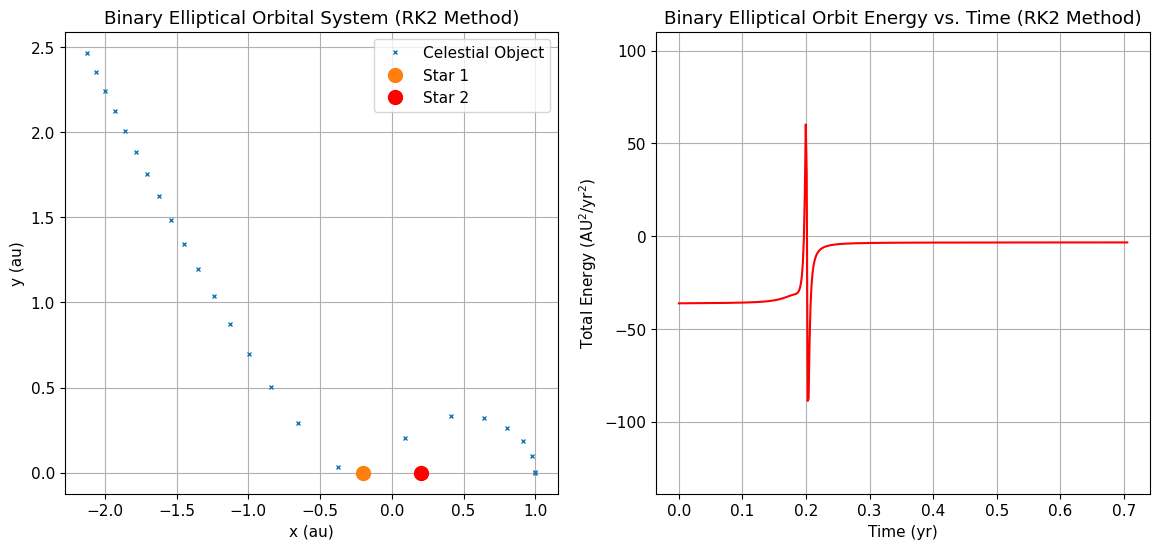
\includegraphics[width=1\linewidth]{binaryrk2elliptic.png}
  \centering
  \caption{\textit{Binary elliptical orbit of the object with $x = 1$ AU and $v_y = \pi$ AU/yr using 
  the RK2 method with its corresponding energy-time graph.}} 
\end{figure}
The orbit rapidly diverges are after a couple of computational steps. Compared to the Euler-Cromer method,
the RK2 method doesn't stay stable for a longer period. The object's trajectory begins to deflect significantly
after approximately 0.2 years, as shown by the sharp variations in the energy-time graph.

Figure 18 shows the elliptical orbit of the object around two stars with the Leapfrog integration method.
\begin{figure}[H]
  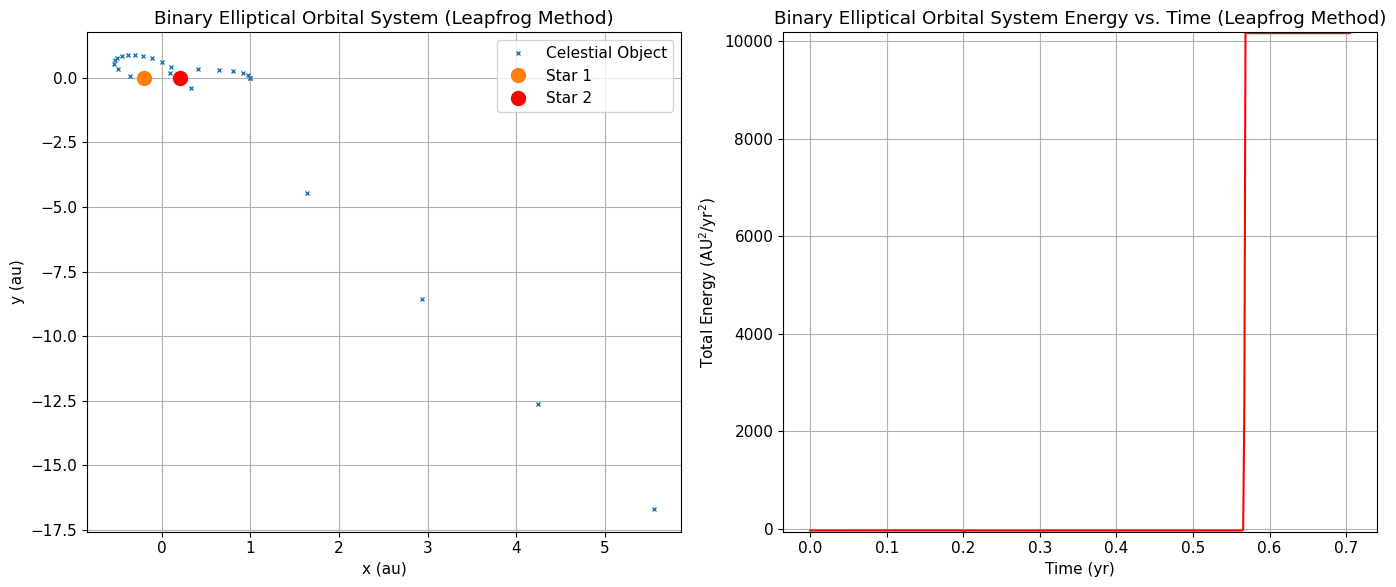
\includegraphics[width=1\linewidth]{binaryleapfrogelliptic.png}
  \centering
  \caption{\textit{Binary elliptical orbit of the object with $x = 1$ AU and $v_y = \pi$ AU/yr using 
  the leapfrog method with its energy-time graph.}} 
\end{figure}
The orbit remains stable for a longer duration compared to the other methods, maintaining the path until
approximately 0.55 years, when the object drifts out of the system. The energy-time graph confirms this
behaviour, showing the stability of the orbit when near the stars, followed by a sudden increase in energy
as the orbit becomes unstable and the object escapes.

\section{Discussion}
The initial conditions provided confirmed Newton's Law of Gravitation and Kepler's Laws. Circular 
orbits were produced at the predicted velocity of $2\pi$ AU/yr at 1 AU, while slower velocities produced
elliptical orbits.

From the three graphs presented for the circular orbits, it can be observed that all three integration 
methods worked well, preserving the law of conservation of energy and angular momentum, as well as maintaining
the orbital shape. The Euler-Cromer method was simple and computationally efficient but accumulated
larger errors at increased time steps. The RK2 method reduced numerical error compared to Euler-Cromer
but lacked long term stability. Circular orbit maintained constant energy, resulting in a steady constant
sum. However, the Euler-Cromer method showed a small dip in the energy-time graph, showing that energy
was not properly conserved at extended periods.

For the elliptical orbits, all numerical methods captured the shape of the trajectory. However, both 
the Euler-Cromer and RK2 methods showed visible deviations over longer periods. The energy-time graphs 
for these methods exhibited energy drifts, with RK2 showing the most deviation. In contrast, the Leapfrog
method demonstrated the most stable orbital behaviour with minimal deviations, effectively conserving the
energy and angular momentum over time. This makes the method the most accurate and stable of the three models.

Changing the time step ($\Delta t$) and the number of snapshots used for computation and plottng had
significant impact on the long term results. For circular orbits, the methods maintained stability and 
energy conservation across small and large time steps, with the Leapfrog method showing highest stability
with minimal deviations. For elliptical orbits, smaller time steps (as used in Section 3.3.1) produced
stable results with good conservation of energy and angular momentum. However, at increased time steps, 
the orbits became unstable, and the object spiraled out of orbit. Energy and angular momentum were only 
conserved in the inital phase of motion. These results demonstrated that increased time steps caused significant
distortion in orbital shape, hence affecting the energy of the system.

The behaviour of the methods in binary systems was also of particular interest. For circular orbits, all
three methods maintained the orbital shape. The Euler-Cromer and RK2 methods showed fluctuations around 
the theoretical energy value, with RK2 performing slightly better. The Leapfrog method, however, 
presented a nearly perfect straight line energy-time graph, preserving energy and angular momentum well.
Circular orbits showed no chaotic behaviour, although some data points suggest that more computational integrations
and longer simulation periods are required for the complete 'picture' of the orbit.

For elliptical orbits in binary systems, the trajectories were more complex, often leading to chaotic
motion and eventually, ejection of the object from the system. Energy conservation proved key for maintaining
stable orbits in this system. The Euler-Cromer and RK2 method did not show stability, while the Leapfrog
method successfully conserved energy for a longer period of time, creating a quasi-elliptical orbit before drifting away.

\section{Conclusion}
This computational lab explored the application of three numerical integration methods = Euler-Cromer, 
2nd Order Runge-Kutta (RK2), and Leapfrog - in simulating orbital motion in a single-star and binary system.
The study verified Newton's Laws of Gravitation and Kepler's Laws of Planetary Motion, successfully
reproducing circular and elliptical orbits under the provided initial conditions.

Among the 3 methods, the Leapfrog methods demonstrated the highest degree of accuracy and long-term stability.
It effectively conserved energy and angular momentum, maintaining orbital shape over extended time periods and
larger time steps. The Euler-Cromer method was simple computationally, but showed larger numerical errors
at higher time steps, and the RK2 method, though initially accurate, failed to sustain over longer periods.

Varying the time step and number of computational snapshots revealed that smaller time steps yielded greater
accuracy and stability, while larger time steps introduced energy drift and orbital distortion. In binary
systems, the complexity of the gravitational forces and the bodies' interactions with it amplified these effects,
with Leapfrog method maintaining a reasonable stability over time.

Overall, the Leapfrog integration method proved to be the most reliable for long-term orbital simulations
due to its symplectic nature, which conserves both energy and angular momentum. Future researches could extend to using
this method to create/modify to create a higher-rder symplectic integrators which can then be used to handle more complex
n-body problems, thereby improving precision, accuracy and reliability.

\section{References}  

[1] NASA. "Chapter 7 Fundamentals of Orbital Mechanics." NASA. Accessed: 19 Sept. 2025. [Online]. Available: \url{https://spsweb.fltops.jpl.nasa.gov/portaldataops/mpg/MPG_Docs/MPG%20Book/Release/Chapter7-OrbitalMechanics.pdf}.

[2] "2.9 Newton's Law of Gravitation - Physics LibreTexts." Physics LibreTexts. Accessed: 19 Sept. 2025. [Online]. Available: \url{https://phys.libretexts.org/Bookshelves/Conceptual_Physics/Introduction_to_Physics_(Park)/02%3A_Mechanics_I_-_Motion_and_Forces/02%3A_Dynamics/2.09%3A_Newtons_Universal_Law_of_Gravitation}

[3] J. J. Lissauer and C. D. Murray, "Chapter 3 - Solar System Dynamics: Regular and Chaotic Motion," in \textit{Encyclopedia of the Solar System} T. Spohn, D. Breuer and T. V. Johnson, Eds., Elsevier, 2014, pp. 55-79. Available: \url{https://www.sciencedirect.com/science/article/pii/B9780124158450000037}

[4] D. Coffey. (2025). Exploring the Solar System [PowerPoint slides].

[5] B. Weber. "Energy Is Conserved In Orbital Motion." Orbital Mechanics \& Astrodynamics. Accessed: 20 Sept. 2025. [Online]. Available: \url{https://orbital-mechanics.space/constants-of-orbital-motion/energy-is-conserved-in-orbital-motion.html}

[6] DIAS. (2009). TP 3:Runge-Kutta Methods-Solar System-The Method of Least Squares. [Online]. Available: \url{https://homepages.dias.ie/ydri/TP3-en.pdf}

[7] A. Cromer, "Stable solutions using the Euler approximation," \textit{Am. J. Phys.}, vol. 49, no. 9, pp. 455-459 May 1981. Accessed: 20 Sept. 2025. [Online]. Available: \url{https://liceocuneo.it/oddenino/wp-content/uploads/sites/2/Alan-Cromer-Stable-solutions-using-the-Euler-Approximation-American-Journal-of-Physics-49-455-1981.pdf}

[8] X. Yang, "Chapter 20 - Numerical Methods," in \textit{Engineering Mathematics with Examples and Applications.} X. Yang, Ed., Academic Press, 2017, pp. 231-241. Available: \url{https://doi.org/10.1016/B978-0-12-809730-4.00027-6.}

[9] M. Ghrist, B. Fornberg and T. A. Driscoll, "Staggered Time Integrators For Wave Equations," \textit{SIAM J. Numer. Anal.}, vol. 38, no. 3, pp. 718-741, Jan. 2000. doi: 10.1137/S0036142999351777. [Online]. Available: \url{https://epubs.siam.org/doi/10.1137/S0036142999351777}
\newpage
\onecolumn
\section{Appendix}

\subsection{Coding}
\subsubsection{The Euler-Cromer Method for a Non-Binary System}
\lstinputlisting[language=Python]{Euler cromer/euleronestar.py}

\subsubsection{The 2nd Order Runge-Kutta Method for a Non-Binary System}
\lstinputlisting[language=Python]{RK2/2rkonestar.py}

\subsubsection{The Leapfrog Method for a Non-Binary System}
\lstinputlisting[language=Python]{Leapfrog/leapfrogonestar.py}

\subsubsection{The Euler Method for a Binary System}
\lstinputlisting[language=Python]{binaryeuler.py}

\subsubsection{The Leapfrog Method for a Binary System}
\lstinputlisting[language=Python]{binaryleapfrog.py}


\end{document}
